\begin{figure}[ht]
  \centering
  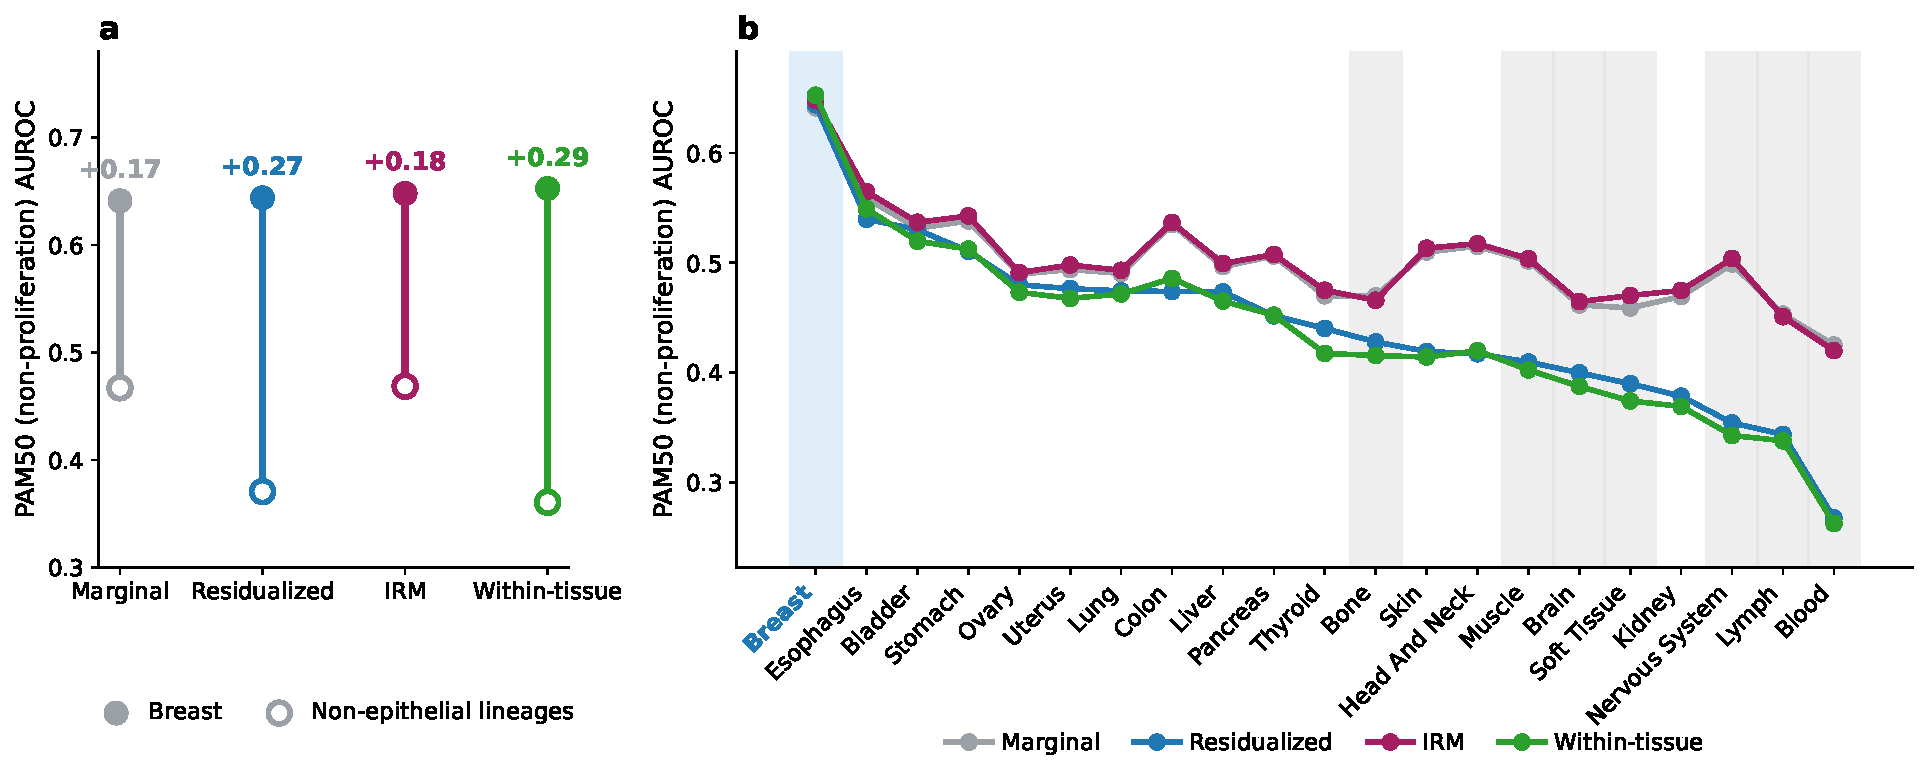
\includegraphics[width=\textwidth]{figures/fig_breast_subtypes.pdf}
  \caption{Deconfounded attribution recovers breast-cancer subtype (PAM50)
  genes specifically in breast (CTRPv2 drug response). For every (drug, tissue)
  pair with $\geq 10$ cell lines, the 1109 panel genes were ranked by mean
  $|\mathrm{SHAP}|$ within that tissue and the ranking was scored by AUROC
  against the 27 non-proliferation PAM50 (Parker 2009) breast-subtype genes in
  the panel (the proliferation arm is uninformative in uniformly-proliferating
  cell lines); tissues covered by $\geq 20$ drugs ($n = 21$) were retained and
  per-tissue AUROCs averaged across drugs. The AUROC should peak in breast and
  be lower in most unrelated, non-epithelial lineages.
  \textbf{a}: Breast-specificity gap per method. Filled markers give PAM50
  recovery in breast, open markers the mean across non-epithelial lineages
  (Blood, Lymph, Muscle, Bone, Soft Tissue, Nervous System, Brain), which should
  not exhibit PAM50-dependent drug response.
  \textbf{b}: Per-tissue PAM50 AUROC for all four methods across the 21 tissues,
  sorted by Residualized. Non-epithelial lineages are shaded grey. Within-tissue
  and Residualized keep the breast signal at full strength while reducing the
  unrelated lineages to or below chance, whereas Marginal and IRM remain inflated
  in most unrelated tissues.%
}
\end{figure}
